\documentclass[11pt, a4paper]{article}
\usepackage{pdfpages}
\usepackage{parallel}
\usepackage[T2A]{fontenc}
%\usepackage{ucs}
\usepackage[utf8]{inputenc}
\usepackage[english,russian]{babel}
\usepackage{hyperref}
\usepackage{rotating}
\usepackage[inner=2cm,top=1.8cm,outer=2cm,bottom=2.3cm,nohead]{geometry}
%\usepackage{listings}
\usepackage{graphicx}
\usepackage{wrapfig}
\usepackage{longtable}
\usepackage{indentfirst}
\usepackage{array}
\usepackage{tikzsymbols}
\usepackage{soul}
\usepackage[ruled,vlined]{algorithm2e}
\usepackage{qrcode}
\counterwithout{figure}{section} 

\usepackage{url}
\makeatletter
\g@addto@macro{\UrlBreaks}{\UrlOrds}
\makeatother

\newcolumntype{P}[1]{>{\raggedright\arraybackslash}p{#1}}
\frenchspacing
%\usepackage{fixltx2e} %text sub- and superscripts
\usepackage{icomma} % коскі ў матэматычным рэжыме
%\PreloadUnicodePage{4}

\newcommand{\longpage}{\enlargethispage{\baselineskip}}
\newcommand{\shortpage}{\enlargethispage{-\baselineskip}}

\def\switchlang#1{\expandafter\csname switchlang#1\endcsname}
\def\switchlangbe{
\let\saverefname=\refname%
\def\refname{Літаратура}%
\def\figurename{Іл.}%
}
\def\switchlangru{
\let\saverefname=\refname%
\let\savefigurename=\figurename%
\def\refname{Литература}%
\def\figurename{Рис.}%
}
\def\switchlangen{
\let\saverefname=\refname%
\def\refname{References}%
\def\figurename{Fig.}%
}

\hyphenation{admi-ni-stra-tive}
\hyphenation{ex-pe-ri-ence}
\hyphenation{fle-xi-bi-li-ty}
\hyphenation{Py-thon}
\hyphenation{ma-the-ma-ti-cal}
\hyphenation{re-ported}
\hyphenation{imp-le-menta-tions}
\hyphenation{pro-vides}
\hyphenation{en-gi-neering}
\hyphenation{com-pa-ti-bi-li-ty}
\hyphenation{im-pos-sible}
\hyphenation{desk-top}
\hyphenation{elec-tro-nic}
\hyphenation{com-pa-ny}
\hyphenation{de-ve-lop-ment}
\hyphenation{de-ve-loping}
\hyphenation{de-ve-lop}
\hyphenation{da-ta-ba-se}
\hyphenation{plat-forms}
\hyphenation{or-ga-ni-za-tion}
\hyphenation{pro-gramming}
\hyphenation{in-stru-ments}
\hyphenation{Li-nux}
\hyphenation{sour-ce}
\hyphenation{en-vi-ron-ment}
\hyphenation{Te-le-pathy}
\hyphenation{Li-nux-ov-ka}
\hyphenation{Open-BSD}
\hyphenation{Free-BSD}
\hyphenation{men-ti-on-ed}
\hyphenation{app-li-ca-tion}

\def\progref!#1!{\texttt{#1}}
\renewcommand{\arraystretch}{2} %Іначай формулы ў матрыцы зліпаюцца з лініямі
\usepackage{array}

\def\interview #1 (#2), #3, #4, #5\par{

\section[#1, #3, #4]{#1 -- #3, #4}
\def\qname{LVEE}
\def\aname{#1}
\def\q ##1\par{{\noindent \bf \qname: ##1 }\par}
\def\a{{\noindent \bf \aname: } \def\qname{L}\def\aname{#2}}
}

\def\interview* #1 (#2), #3, #4, #5\par{

\section*{#1\\{\small\rm #3, #4. #5}}
\ifx\ParallelWhichBox\undefined%
    \addcontentsline{toc}{section}{#1, #3, #4}%
\else%
\ifnum\ParallelWhichBox=0%
    \addcontentsline{toc}{section}{#1, #3, #4}%
\fi\fi%

\def\qname{LVEE}
\def\aname{#1}
\def\q ##1\par{{\noindent \bf \qname: ##1 }\par}
\def\a{{\noindent \bf \aname: } \def\qname{L}\def\aname{#2}}
}

\newcommand{\interviewfooter}[1]{
\vskip 1em
\noindent \textit{#1}
}

\AtEndDocument{\vfill\centering \qrcode{https://github.com/fiowro/mouses/blob/main/\jobname.pdf}}

\switchlang{ru}
\begin{document}

\title{1986 "--- Honeywell/Asher quadLYNX trackball}
\date{}
\maketitle
\selectlanguage{russian}
Трекбол quadLYNX, показанный на рис. \ref{fig:quadLYNXPic}, является модификацией трекбола LX200, разработанной для компьютеров Apple Macintosh. LX200, более известный своими разновидностями microLYNX и comLYNX, был выпущен в калифорнии компанией Honeywell, дочерним предприятием Disc Instruments; он оказался долгожителем и в дальнейшем выдержал множество переизданий под разными брэндами, отличаясь интерфейсом подключения и блоком электроники \cite{lx200}. Рекламные материалы позволяют датировать модель quadLYNX под брэндом Honeywell 1986 годом \cite{honeywell}. Однако в 1988 году появляется похоже оформленная реклама данной модели как <<LX200-192-D1>> под брэндом Asher Engineering Corporation (с упоминанием Honeywell в качестве изначального разработчика устройства) \cite{asher}. В дополнение к путанице, в том же году Asher Engineering Corporation рекламирует устройство Turbo Trackball --- исключительно под собственным брэндом, в корпусе другой формы, но с сильным сходством в номере модели (<<LX200-192-S3A>>) и части внутренних конструктивных решений \cite{turbo}.

\begin{figure}[h]
    \centering
    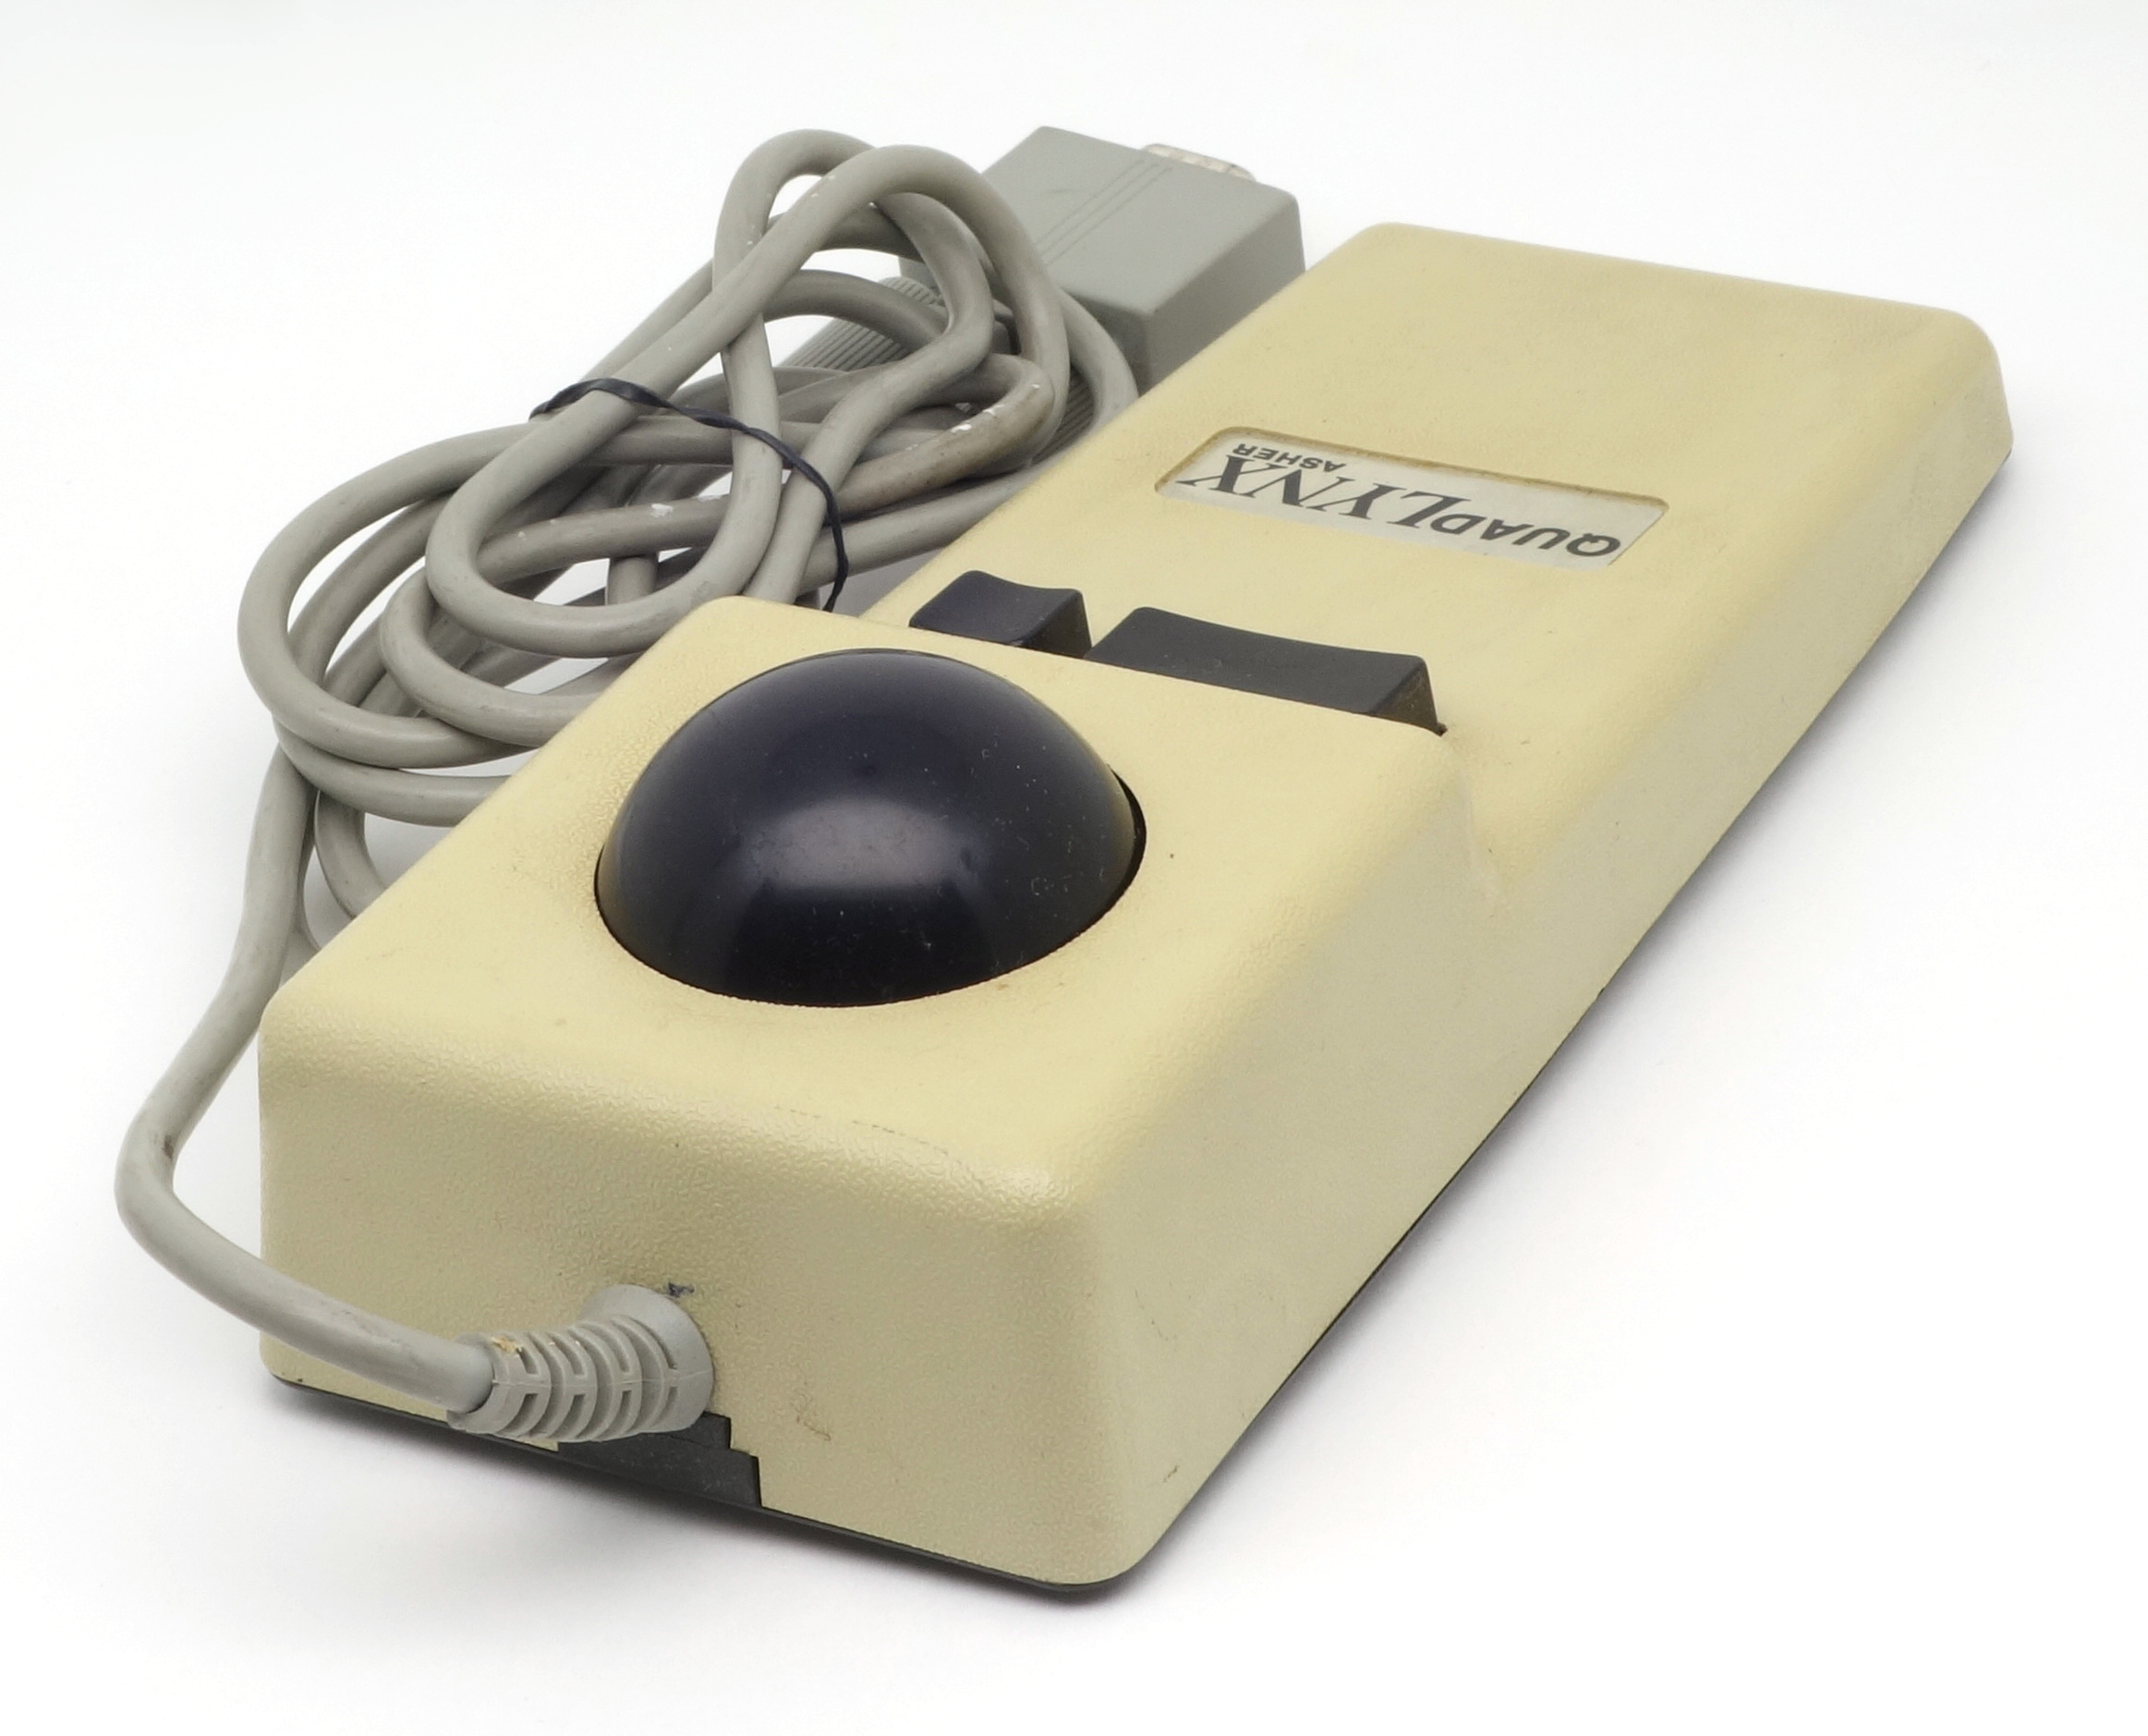
\includegraphics[scale=0.75]{1986_honeywell_asher_quadlynx_trackball/pic_30.jpg}
    \caption{Внешний вид трекбола quadLYNX}
    \label{fig:quadLYNXPic}
\end{figure}

Трекбол выполнен в характерном для LX200 дизайне, с большим черным шаром, утопленным в бежевом корпусе, и вытянутой подставкой под запястье \ref{fig:quadLYNXTopBottom}. Шар плотно прилегает к краям отверстия в корпусе, что неплохо защищает от попадания мусора внутрь трекбола, но делает извлечение шара для чистки невозможным без разборки корпуса. Перед шаром расположены две кнопки, копирующие внешним видом клавиши классической полноразмерной клавиатуры. Это главное визуальное отличие quadLYNX от других вариантов LX200, оснащенных тремя кнопками.

\begin{figure}[h]
    \centering
    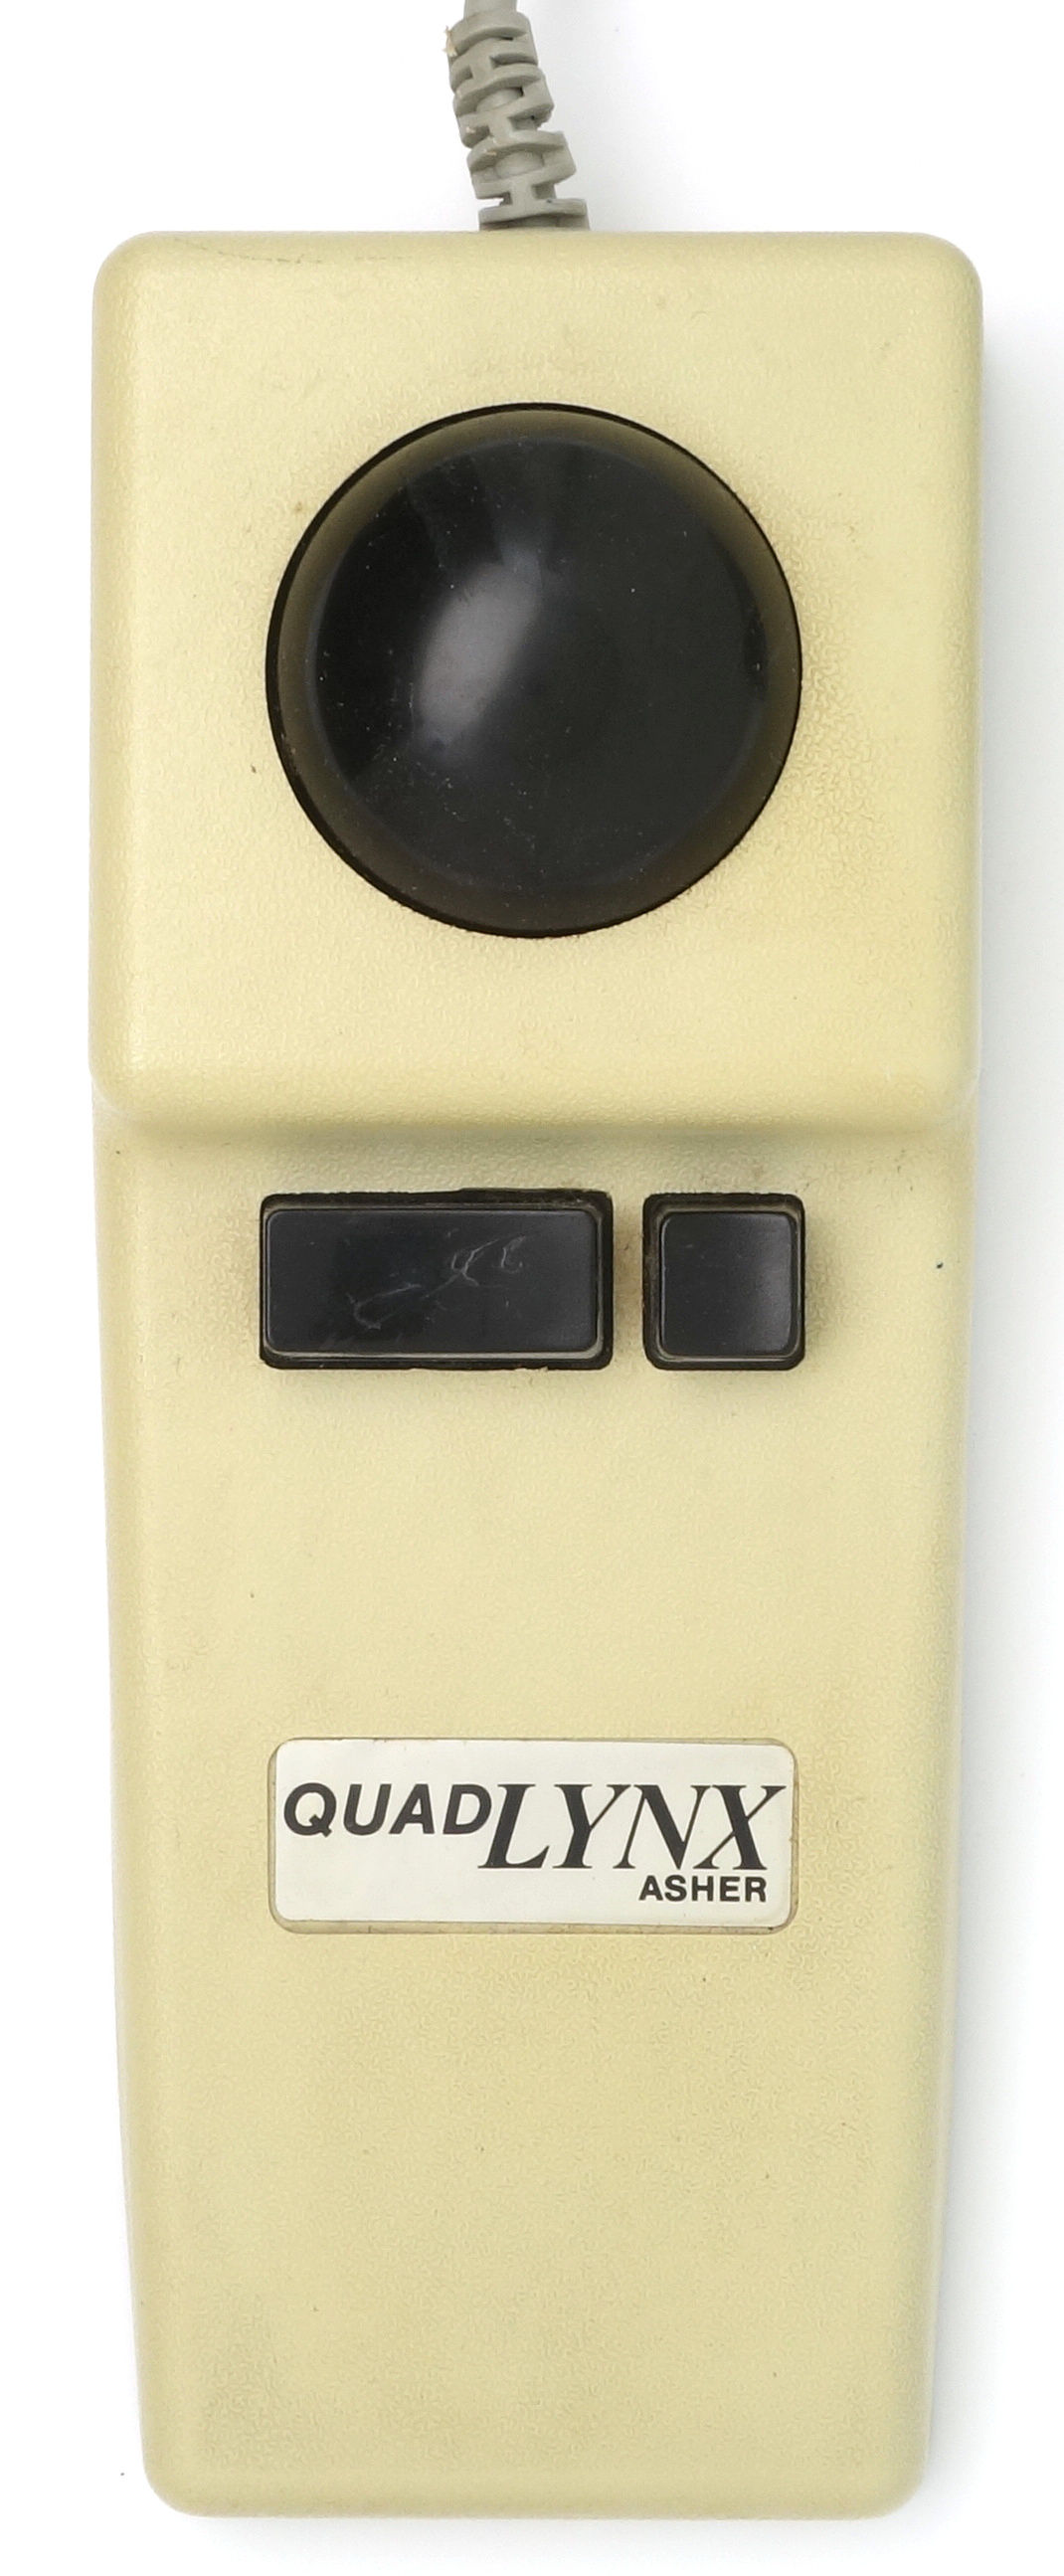
\includegraphics[scale=0.41]{1986_honeywell_asher_quadlynx_trackball/top_30.jpg}
    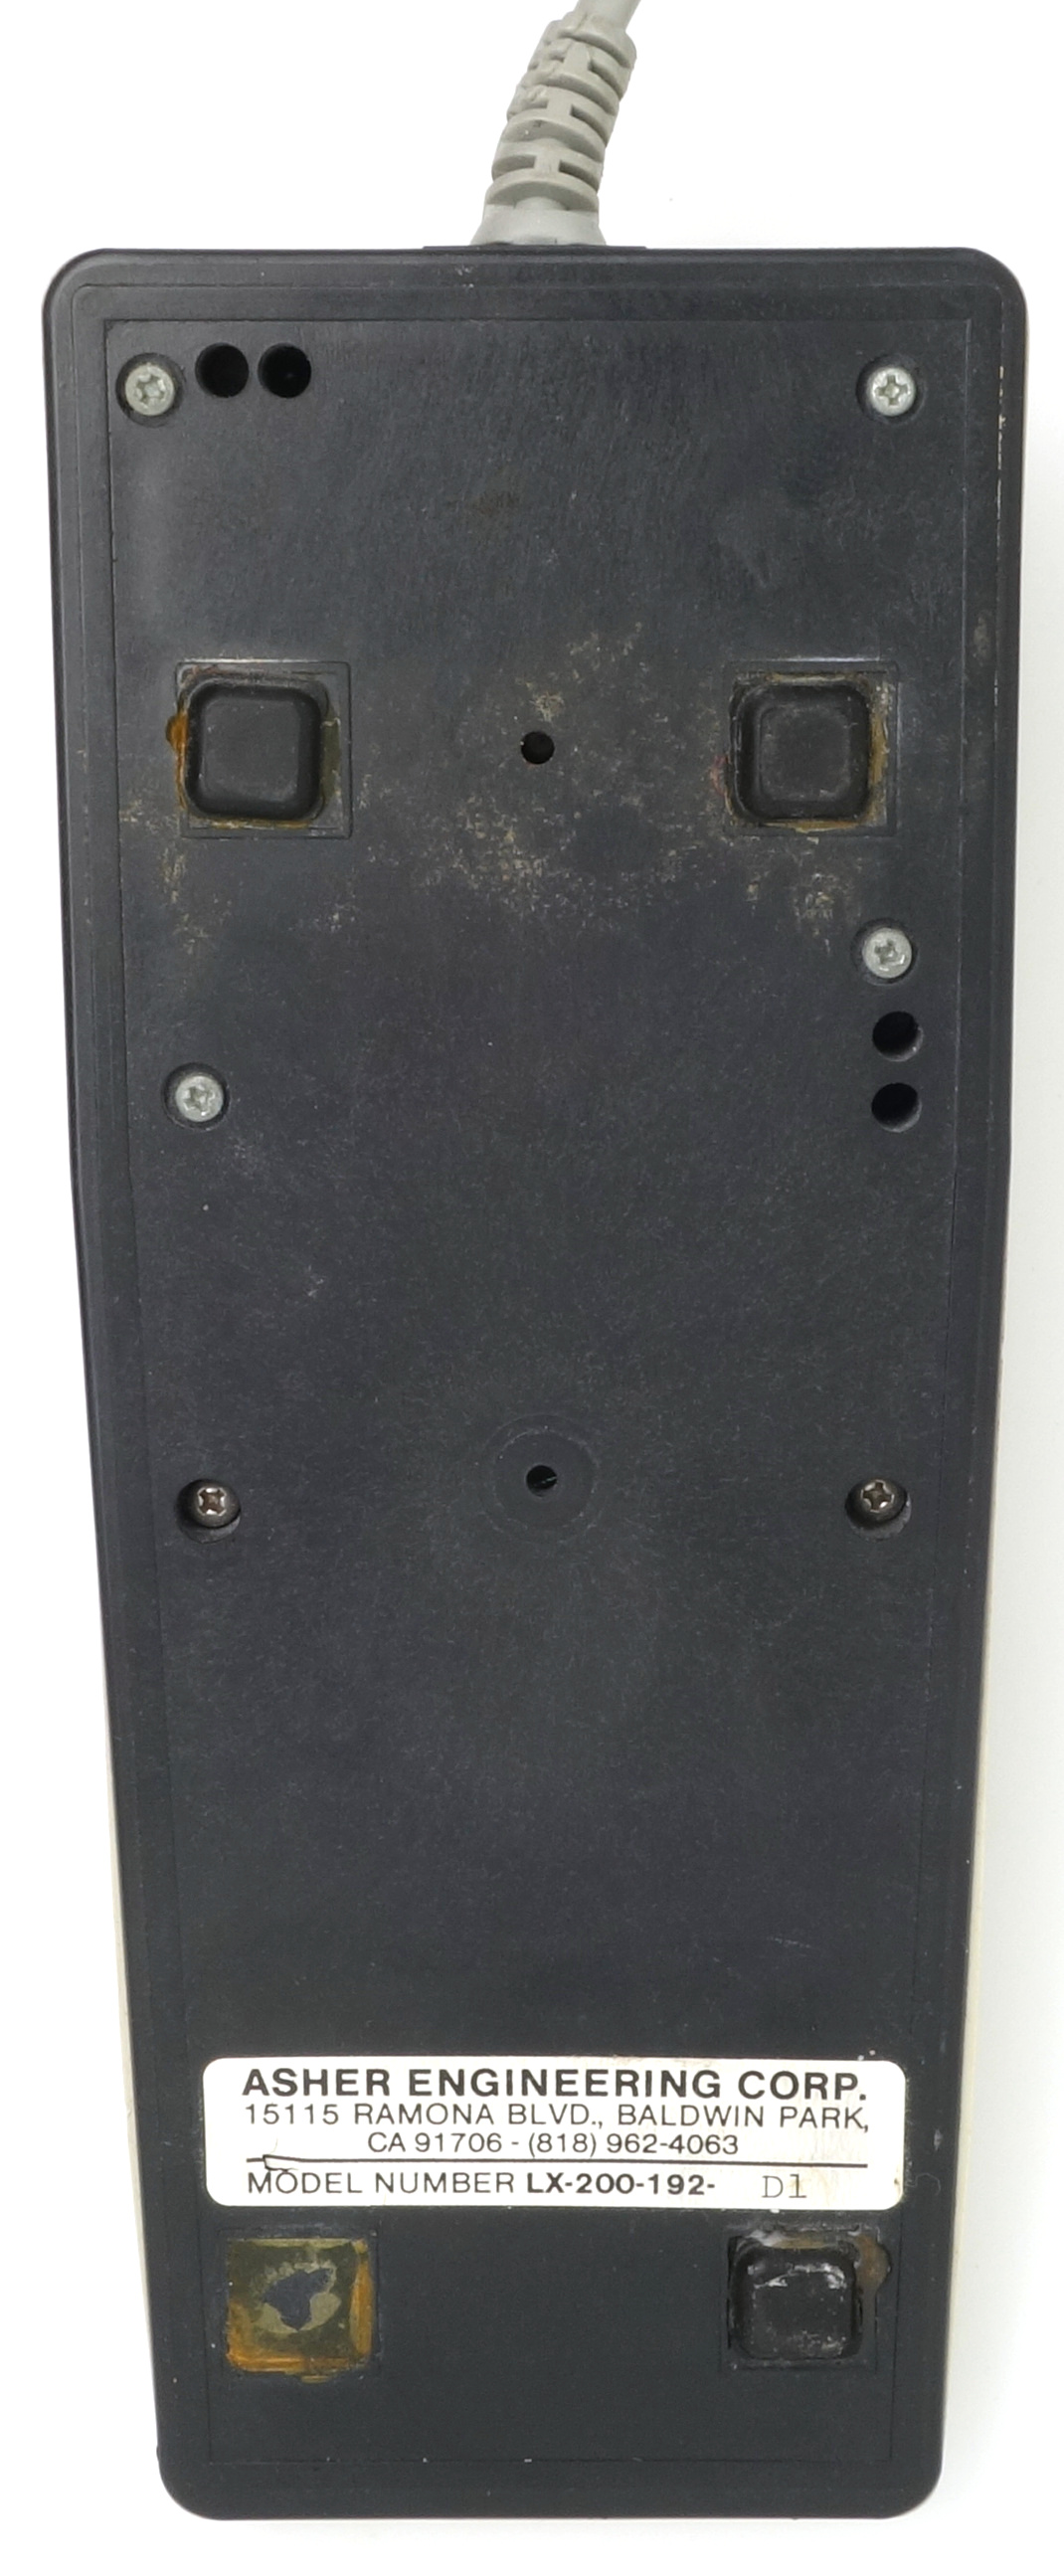
\includegraphics[scale=0.41]{1986_honeywell_asher_quadlynx_trackball/bottom_30.jpg}
    \caption{quadLYNX, вид сверху и снизу}
    \label{fig:quadLYNXTopBottom}
\end{figure}

В отношении эргономики размеры трекбола (рис. \ref{fig:quadLYNXSize}), а также скругленные грани и углы, могли бы создавать достаточно комфортные условия для работы.

\begin{figure}[h]
    \centering
    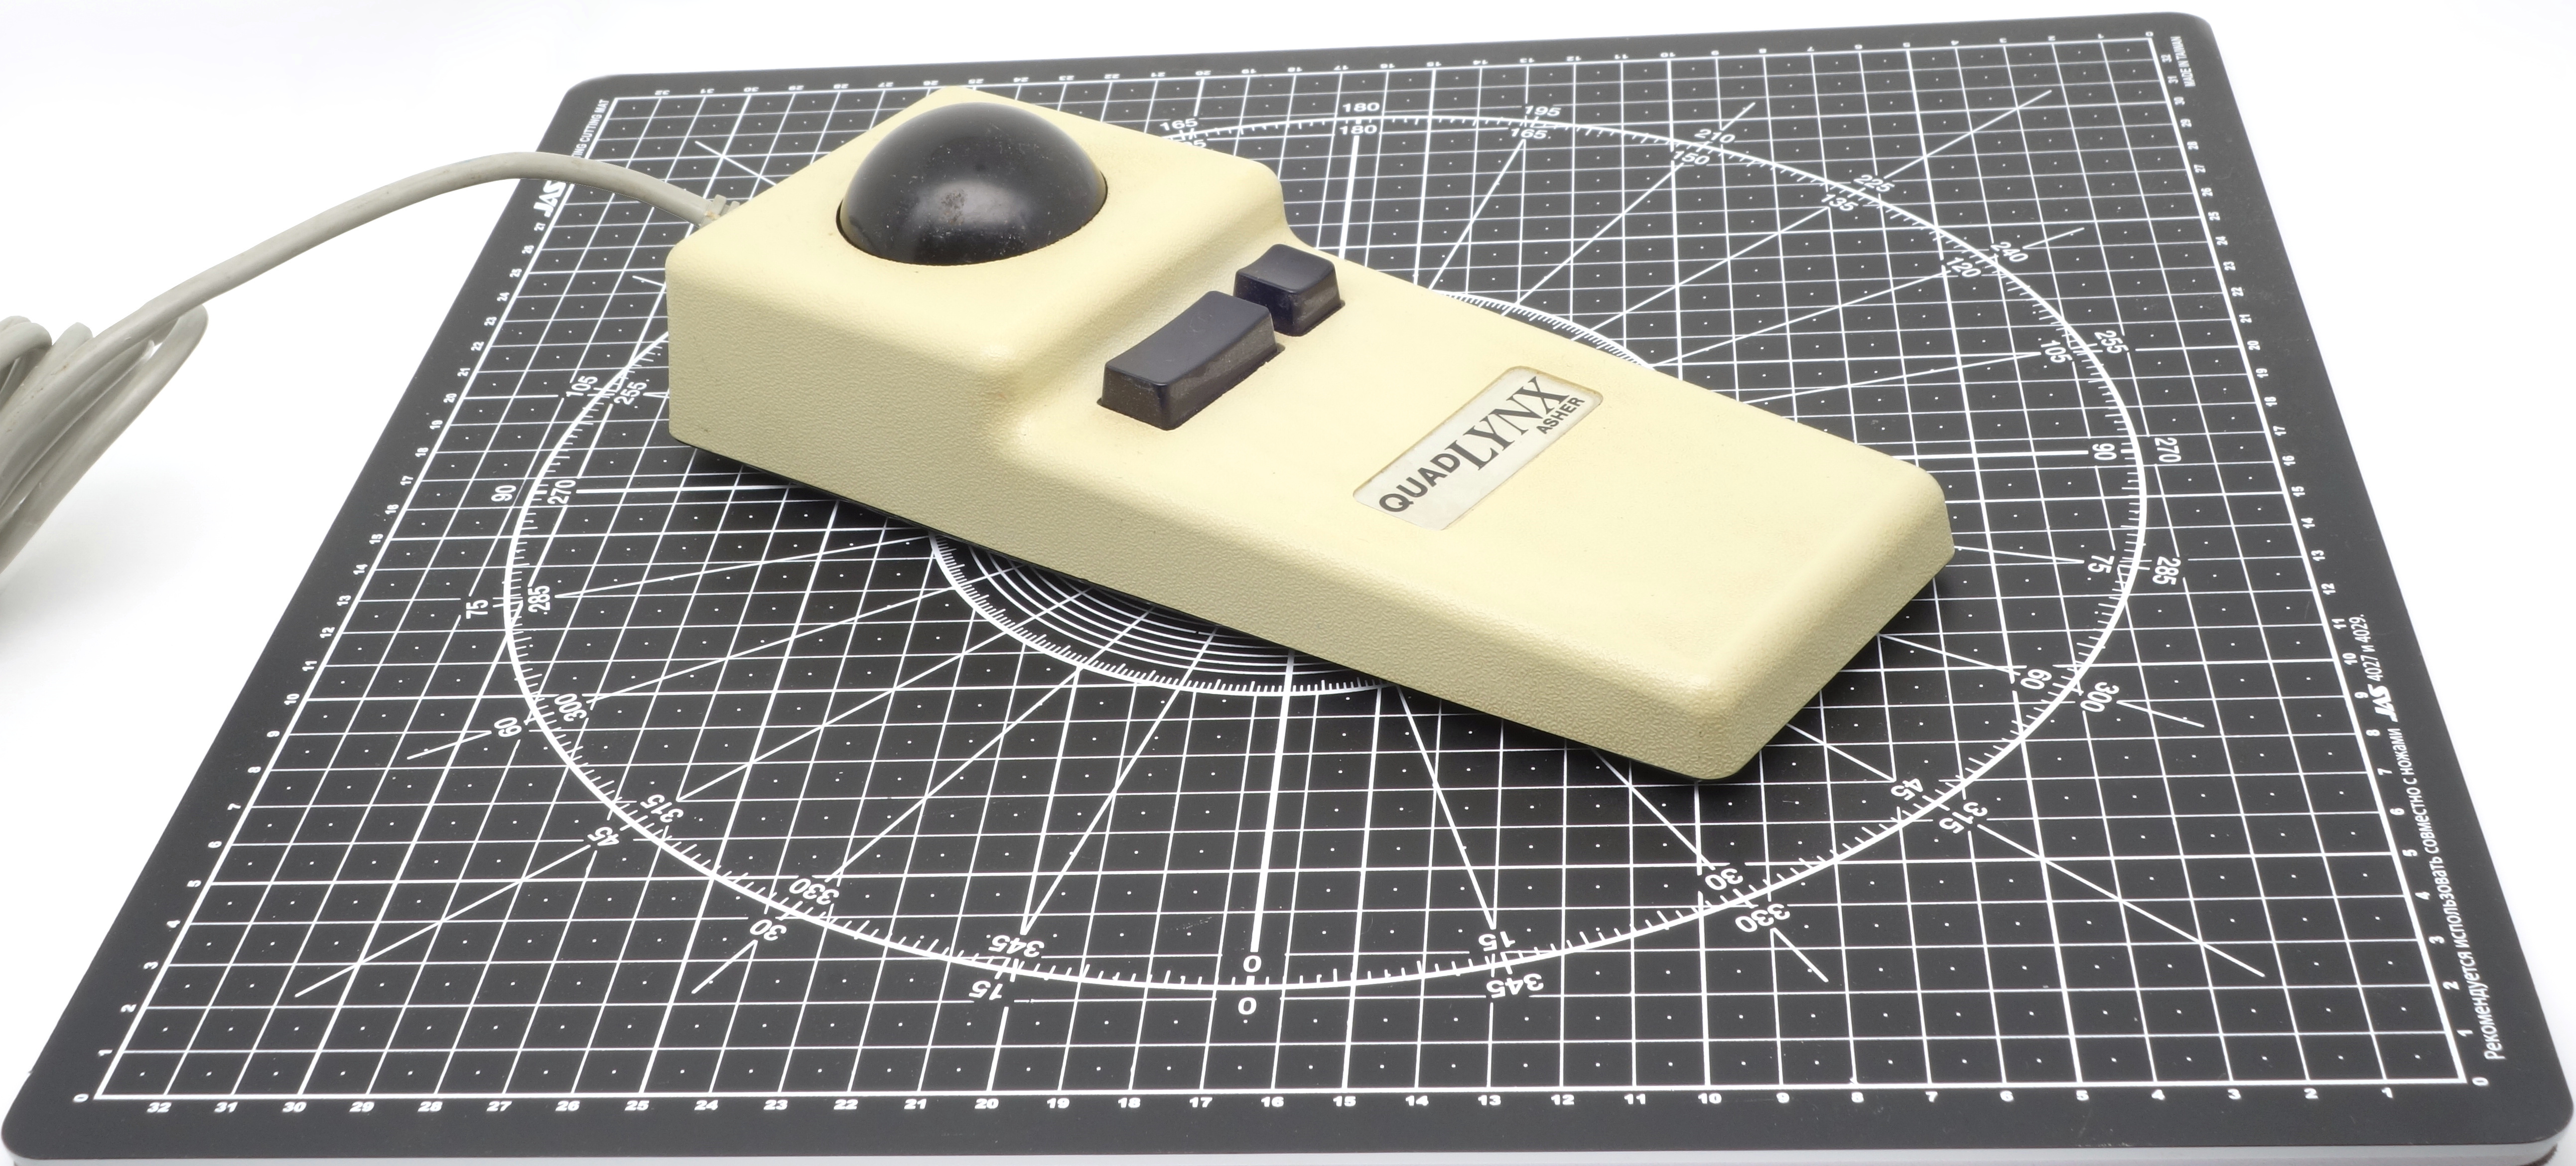
\includegraphics[scale=0.4]{1986_honeywell_asher_quadlynx_trackball/size_30.jpg}
    \caption{Трекбол quadLYNX на размерном коврике с шагом сетки 1 см}
    \label{fig:quadLYNXSize}
\end{figure}

Однако кнопки расположены далеко от шара  и область их расположения находится существенно ниже, что лишает пользователя как возможности нажимать их одной рукой без перемещения кисти, так и двумя руками, поскольку при вращении шара они закрыты ладонью (рис. \ref{fig:quadLYNXHand}). Особенно это затрудняет перетаскивание объектов, повсеместно использовавшееся в интерфейсе компьютеров Macintosh, для которых предназначался трекбол. Чтобы уменьшить проблему, правая меньшая по размеру кнопка работает в качестве <<защелки>> перетаскивания. Нажатие кнопки-защёлки программно фиксирует основную кнопку трекбола в нажатом положении, а повторное нажатие любой из кнопок отключает данный режим \cite{bible}.

\begin{figure}[h]
    \centering
    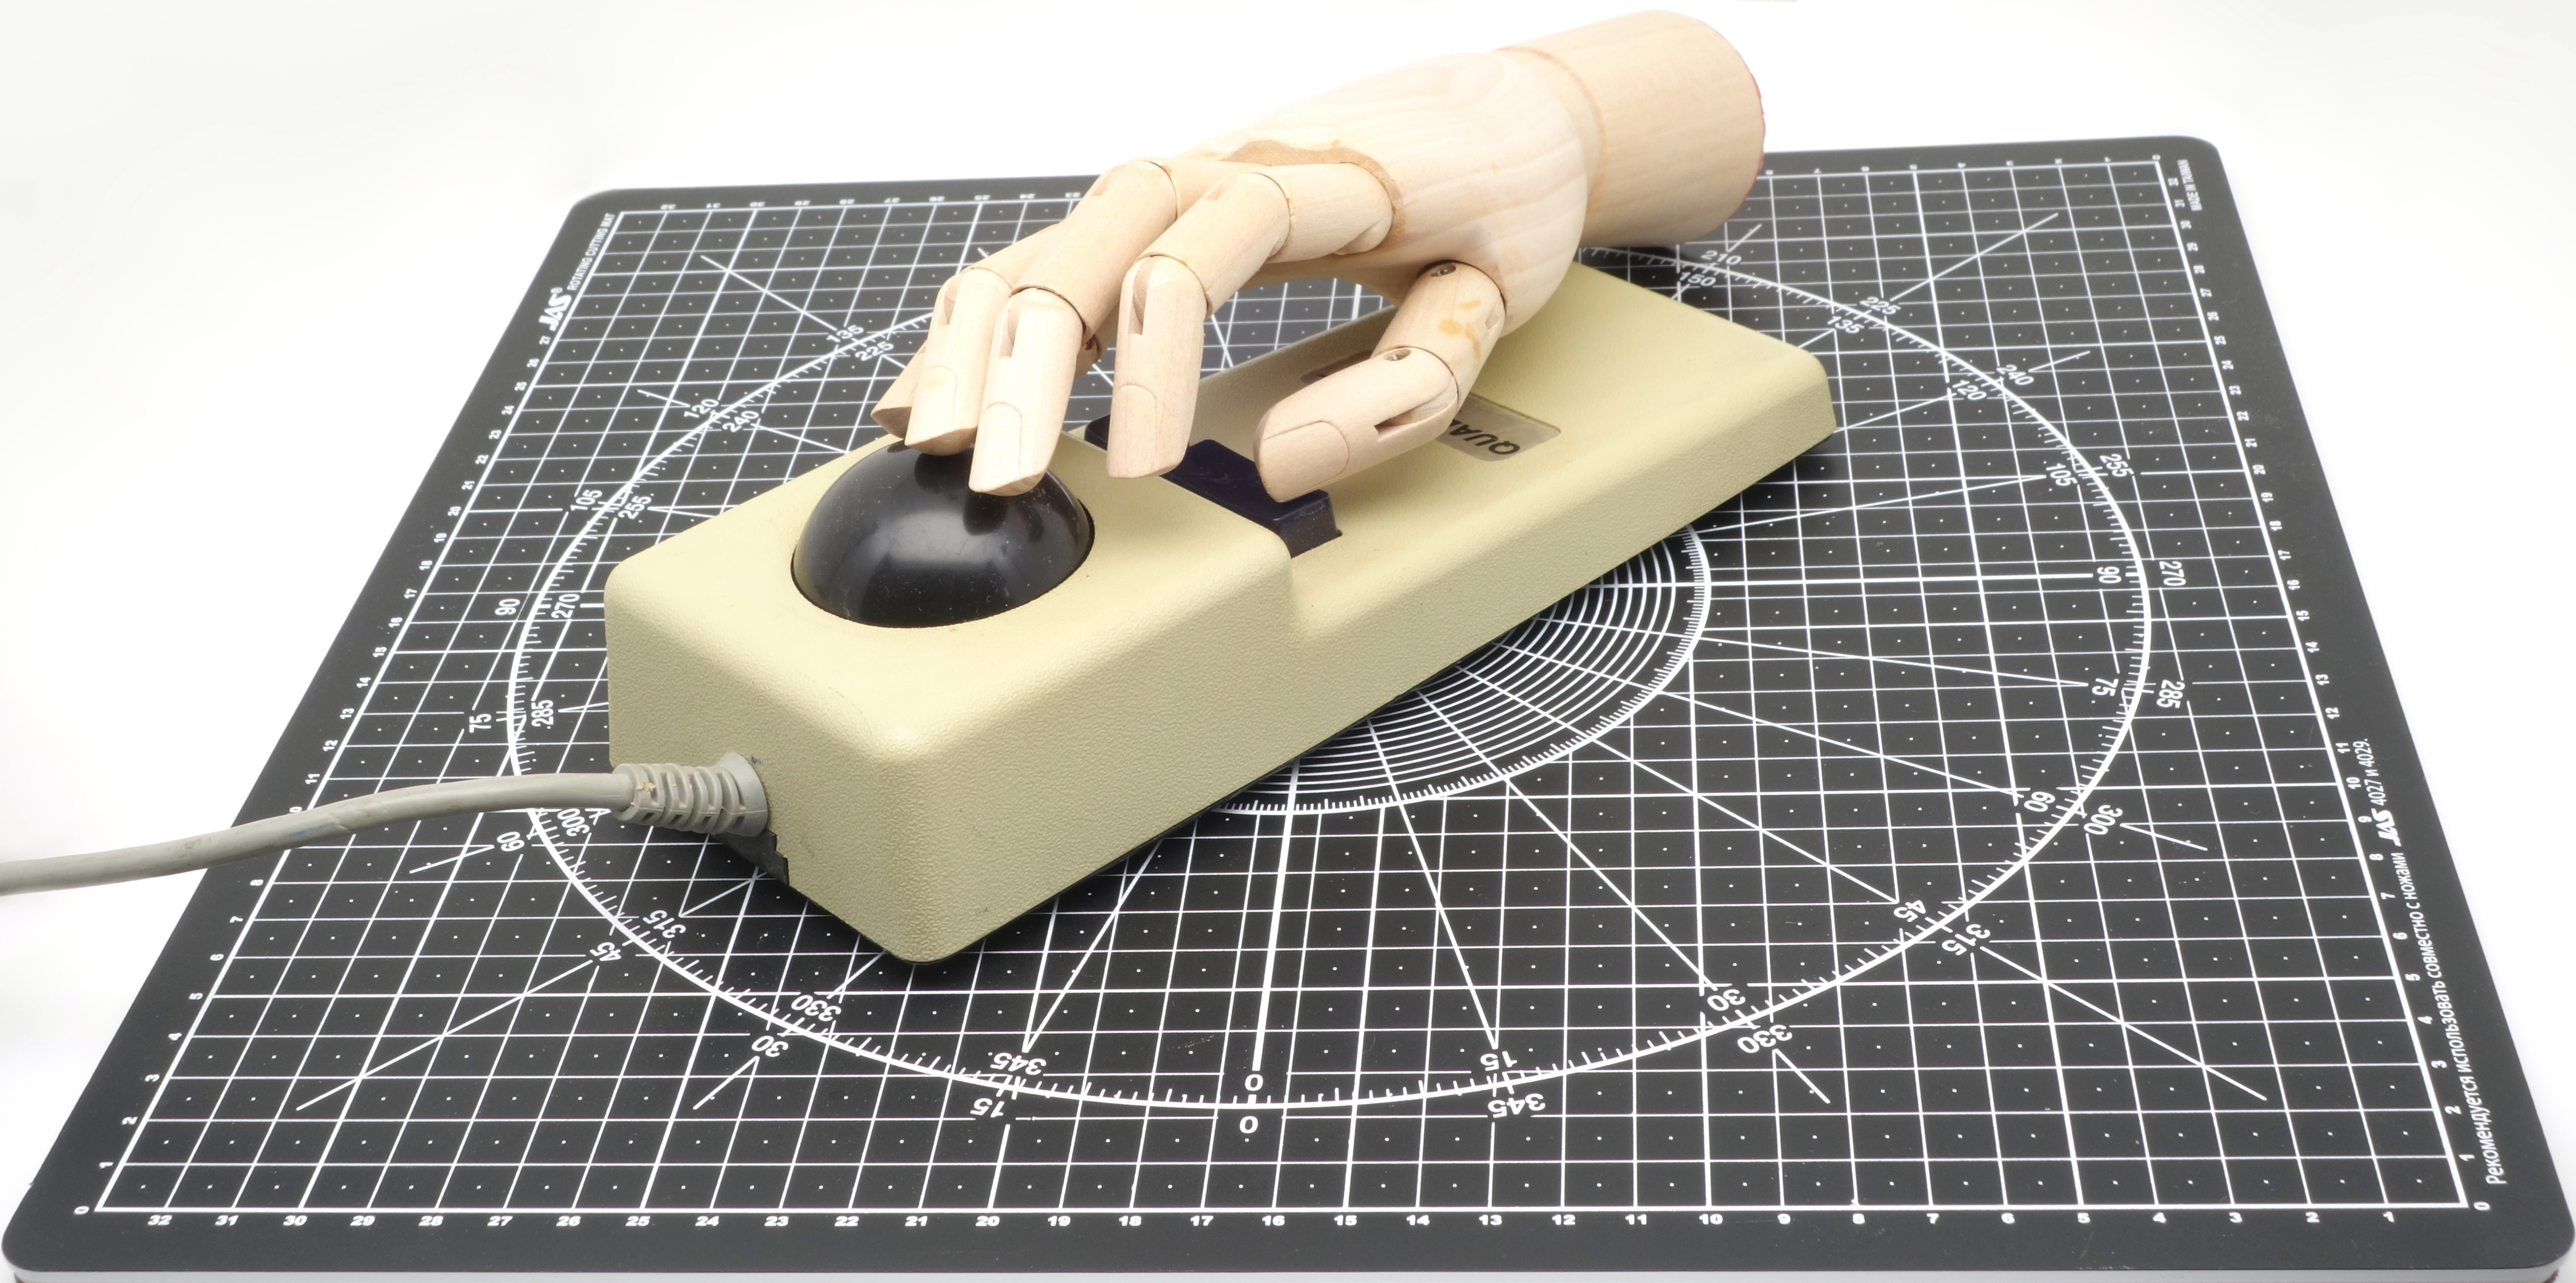
\includegraphics[scale=0.4]{1986_honeywell_asher_quadlynx_trackball/hand_30.jpg}
    \caption{Трекбол quadLYNX в комплекте с моделью руки человека}
    \label{fig:quadLYNXHand}
\end{figure}

Внутреннее устройство данного трекбола показано на рис. \ref{fig:quadLYNXInside}. Он представляет собой устройство с механическим энкодером, в отличие от большинства вариантов LX200, оснащавшихся оптомеханическим энкодером начания с того же самого 1986 года. Согласно информации, приведенной в \cite{lx200}, механический энкодер иногда встречается в ранних экземплярах LX200;  кроме того, такой же реализацией <<запатентованный высокотехнологичный кодер, используемый в сложных аэрокосмических приборах>> \cite{turbo} оснащены трекболы Asher Turbo Mouse 1988 года выпуска. 

Как можно видеть, <<запатентованный высокотехнологичный энкодер>> представляет собой обычный диск механичекого энкодера, накрытый сверху пластмассовой коробочкой, затрудняющей проникновение мусора (при этом его конструкция не настолько герметична и заметно менее технологична по сравнению, например, с закрытыми механическими энкодерами фирмы ALPS Electric, используемыми в ранних моделях мышей Microsoft, IBM и некоторых других компаний).

\begin{figure}[h]
    \centering
    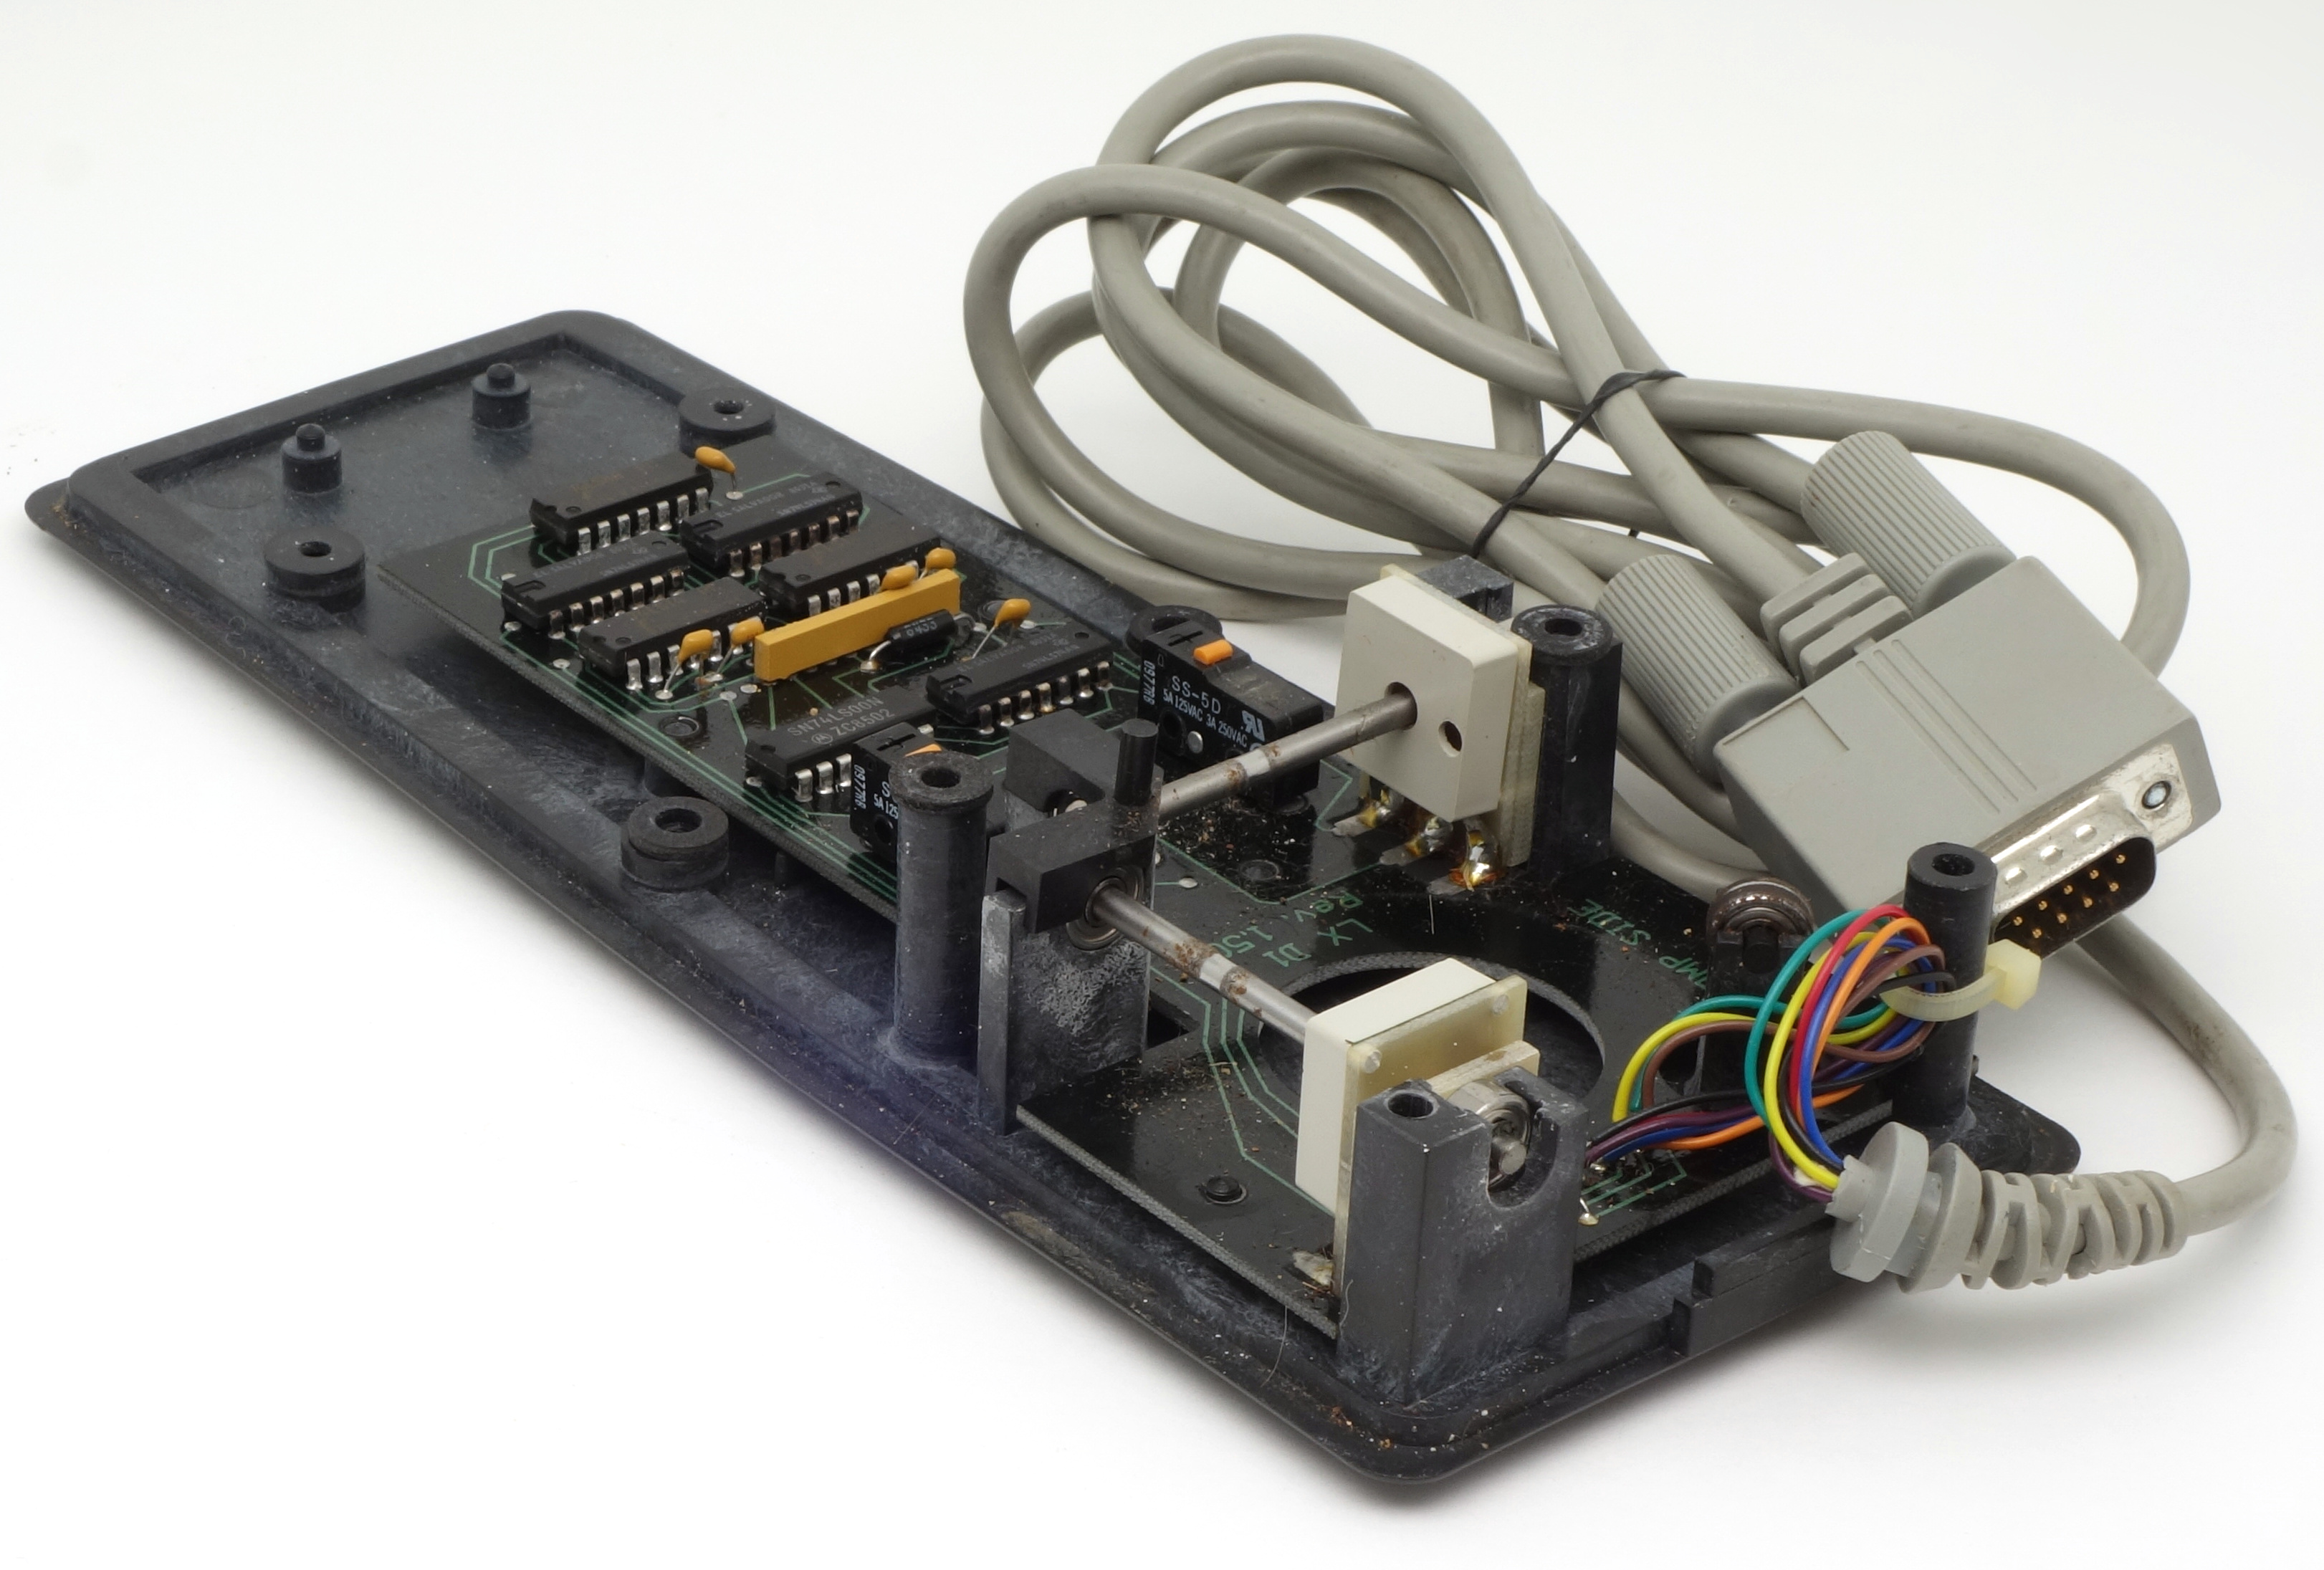
\includegraphics[scale=0.6]{1986_honeywell_asher_quadlynx_trackball/inside_30.jpg}
    \caption{quadLYNX в разобранном виде}
    \label{fig:quadLYNXInside}
\end{figure}

Вероятно, использование механического энкодера вместо оптомеханики было нацелено на удешевление устройства. Однако остальная часть остались без изменений: ролики по-прежнему реализованы с использованием подшипников и валов из нержавеющей стали, обеспечивающих высокую надежность и долговечность механической части устройства.

\begin{thebibliography}{9}
\bibitem {comlynx} Trackballs: Stationary mice // PC Magazine. August 1987, page 199-202 \url{https://trackballs.eu/media/Fulcrum/PC%20Mag%20Aug-1987%20p199-202.pdf}
\bibitem {lx200} Disc Instruments LX200 \url{https://web.archive.org/web/20220501213039/https://forum.trackballs.eu/viewtopic.php?f=17&t=16}
\bibitem {honeywell} Try the new quadLYNX Trackball // Macworld, August 1986. P. 155  \url{https://archive.org/details/eu_Macworld-1986-08_OCR/page/n155/mode/2up}
\bibitem {asher} Try the new quadLYNX Trackball // Macworld, January 1988. P. 212 \url{https://archive.org/details/macworld00unse_oel/page/212/mode/2up}
\bibitem {turbo} New Turbo Trackball from Asher // MacUser, February, 1988. P. 320 
\url{https://archive.org/details/MacUser8802February1988/page/n323/mode/2up}
\bibitem {bible} A. Naiman (ed.) QuadLYNX Trackball, Turbo Mouse. The Macintosh Bible. Chapter 2 -- Basic Mac hardware. PP. 73-75. \url{https://archive.org/details/macintoshbibleth00naim/page/72/mode/2up}
\end{thebibliography}
\end{document}
